\chapter{Grafická časť aplikácie (frontend)}
V rámci frontend časti aplikácie boli použité aplikácie:\begin{itemize}
\item \textbf{QT4 designer} - softvér na nábrh dizajnu "okien" aplikácie
\item \textbf{PyQT 4} - doplnok do pythonu, na návrh a programovenie grafických aplikácií
\end{itemize} 
\section{QT4 disigner}
QT4 designer je aplikácia na návrh šablón v rámci použitia knižnice PyQT4. Medzi základné objekty použité v aplikácii sem patria:
\begin{itemize}
\item \textbf{QPushButton} - tlačítko v GUI
\item \textbf{textlabel} - popis pri tlačítkach a textových poliach
\item \textbf{textedit} - pole na text, obsahuje metódy napr. \textit{text()}
\item \textbf{QListWidget} - časté použitie v aplikácii, napr. pri použití zobrazenia prvkov po stalčení tlačítka, správa prvkov v objekte,objekt je klikateľný, editovateľný, ...
\item \textbf{lineedit} - textové pole na editáciu riadku
\end{itemize} 
Po vytvorení šablóny sa súbor uloží vo formáte \textit{.ui} a musí sa nahrať do kódu aby sa s ním dalo pracovať pomocou príkazu \textit{qtCreatorFile = "súbor.ui"}
\section{PyQT 4}
V aplikácii je použitá verzia PyQT vo verzii 4. Dnes existuje v dvoch verziách a to vo verzii 4 a vo verzii 5. Nakoľko QT4 designer je navrhnutý na PyQT vo verzii 4, tak aj PyQT je v kóde použité vo verzii 4. \\
V rámci okna po prihlásení na zariadenie je okno založené na objekte \textit{menubar()} a na metódach \textit{addMenu()} na pridávanie hlavných položiek v menu a ďalšie položky sú QAcion, ktoré vytvárajú podzložku v menu cez metódu \textit{addAction()}. Ďalšou dôležitou knižnicou je QtGui na vytvorenie GUI plikácie. Objekt \textit{QApplication()} vytvorí samostatnú aplikáciu spoločne s metódou pre otvorenie okna \textit{show()}, tiež je tu použitá knižnica \textit{sys} a jej metóda \textit{exit()} na zatvorenie celej aplikácie,  a ďalšou metódou je \textit{close()}, táto metóda okno zavre.
\chapter{Grafická aplikácia}
\section{Hlavné prihlasovavie okno}
Hlavné okno aplikácie predstavuje prihlasovaciu obrazovku a možnosť zobrazenia blízkych zariadení a to ich IP adries pomocou tlačítka \textit{find devices IP}(vyhľadávacia doba je 30 sekúnd), pomocou tohoto tlačítka sa vylistujú blízke mikrotik zariadenia a ich IP adresy, toto vychádza z aplikácie mactelnet a výstup zachytáva \textit{listIpValues}.\\
Podobne ako zobrazenie IP adries sa pomocou tlačítka find devices MAC (doba hľadania zariadení je 30s sekúnd) vylistuje zoznam MAC adries blízkych zariadení. Pre funkčnosť týchto tlačítok je potreba na linuxe správne nastaviť forward pravidlona firewalle. Podobne ako find devices IP aj toto tlačítko pracuje s programom mactelnet a výstup zachytáva objekt \textit{listMacValues}. Toto vidíme na obrázku \ref{fig:winboxlinux}\\
\begin{figure}[H]
\centering
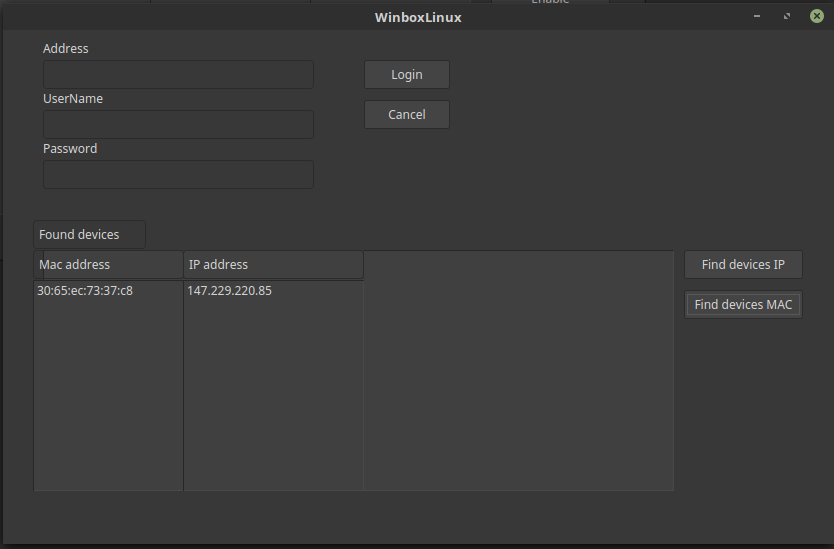
\includegraphics[scale=0.45]{../text/linuxwinbox.png}
\caption{Prihlasovacie okno aplikácie}
\label{fig:winboxlinux}
\end{figure}
Ďalej sa tu nachádzajú textové polia address, username a password. Do týchto polí sa zapisuje IP adresa (je možné ju skopírovať z Ip address textového poľa) zariadenia na ktoré sa chceme pripojiť, užívateľské meno  a heslo a po stlačení tlačítka \textit{login} sa užívateľ pri úspešnom pokuse prihlási na mikrotik pomocou \textit{API-SSL}. V opačnom prípade sa vyhodí okno s výnimkou. Pri nepodpore zariadenia API-SSL prípadne španej komunikácie v rámci overovania certifikátu sa vyhodí nasledujúca výnimka na obrázku \ref{fig:socket}.
\begin{figure}[H]
\centering
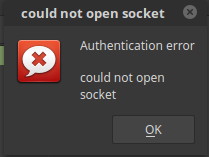
\includegraphics[scale=0.55]{../text/socket.png}
\caption{Výnimka pri španej komunikácii s routrom}
\label{fig:socket}
\end{figure}
Druhým typom výnimky je neúšpešné prihlásenie chybného užívateľského mena alebo hesla. Toto vidíme na obrázku \ref{fig:loginworong}.
\begin{figure}[H]
\centering
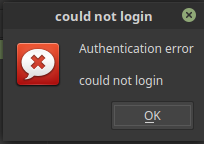
\includegraphics[scale=0.55]{../text/loginerror.png}
\caption{Výnimka pri zadaní zlého užívateľského mena alebo hesla}
\label{fig:loginworong}
\end{figure}
Všetky tieto výnimky sú spravované pod štandardnými výnimkami programovacieho jazyka python a používajú štandardne \textit{try except}.
\subsection{Hlavné okno konfiguračnej aplikácie}
Po úspšnom prihlásení na zariadení sa otvorí okno popisujúce na obrázku \ref{fig:loginokno}.
\begin{figure}[H]
\centering
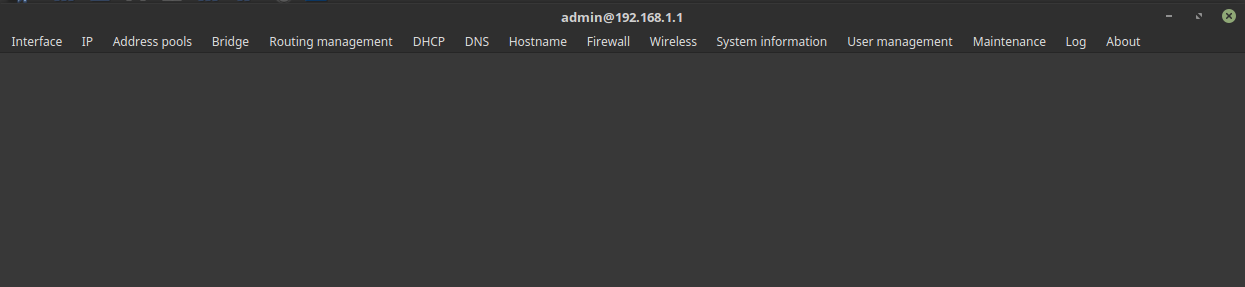
\includegraphics[scale=0.35]{../text/loginokno.png}
\caption{Hlavné okno aplikácie}
\label{fig:loginokno}
\end{figure}
\newpage
\section{Položky hlavného menu}
V menu sa nachádzajú jednotlivé položky a ich podzložky:
\begin{itemize}
\item \textbf{Interface} - správa a manažment rozhraní, pridávanie, odoberanie rozhraní, zapnutie a vypnutie rozhraní, obshauje tiež správu ethernet rozhraní, VLAN rozhraní a tzv. interface listov a ich členov
\item \textbf{IP} - predstavuje správu Ip adries, ARP a služieb na zariadení
\item \textbf{Address pools} - predstavuje správu adries na priraďovanie tzv, adresných rozsahov (poolov)
\item \textbf{Bridge} - predstavuje sprívu bridge rozhrania, VLAN rozhraní, portov bridgu, a pripojených zariadení
\item \textbf{Routing management} - predstavuje správu statického smerovania, susedov, a next-hop zariadení
\item \textbf{DHCP} - predstavuje správu DHCP serveru, klienta a relay, pripojených zariadení na konkrétny server
\item \textbf{DNS} - predstavuje správu nastavenia DNS serverov, správa cache pamäti a statických záznamov
\item \textbf{Hostname} - predstavuje nastavenie systémového mena (hostname)
\item \textbf{Firewall} - predstavuje správu NAT a Filtrovacích pravidiel na vstup a výstup zariadenia, pridávanie povolenia, zakázania  a odmietnutia paketu, správu servisných portov a pripojení, tiež správu tzv. \textit{address listov}
\item \textbf{Wireless} - predstavuje nastavenie bezdrôtovej siete, nastavenie WPA2-PSK profilu na bezdrótové spojenie  a správu pripojených zariadení
\item  \textbf{System information} - predstavuje zobrazenie informácií o procesore,  ovládačoch, diskoch, atď.
\item \textbf{User management} - predstavuje správu užívateľov a zobrazenie pripojených užívateľov
\item \textbf{Maintenance} - predstavuje upgrade, reset zariadenia, obnova konfigurácie, reštart a vypnutie zariadenia
\item \textbf{Log} - predstavuje výpis systémového logu
\item \textbf{About} - predstavuje dve tlačítka Quit a About, About vypíše informácie o softvéri, stalčením tlačítka  Quit sa vypnú všetky okná a celé spojenie zahrňujúc prihlasovacie okno 
\end{itemize}
\subsection{Ukážka fungovania aplikácie cez menu Interface}
Tlačítko interface obsahuje:
\begin{itemize}
\item \textbf{Interfaces} - obsahuje zoznam rozhraní, zapnutie a vypnutie rozhraní spoločne s výnimkami zobrazené na obrázku \ref{fig:interfacesgui} 
\item \textbf{Ethernet} - obsahuje zoznam ethernet rozhraní, zapnutie a vypnutie rozhrania, reset MAC adresy rozhrania zobrazené na obrázku \ref{fig:ethernet}
\item \textbf{VLAN} - obsahuje zoznam VLAN rozhraní, pridanie, odstránenie, zapnutie a vypnutie rozhrania zobrazené na obrázku \ref{fig:vlangui}
\item \textbf{Interface list members} - obsahuje zoznam členov interface listu, ich pridávanie a odstránenie zobrazené na obrázku \ref{fig:interfacelistmembergui}
\item \textbf{Interface lists} - predstavuje zoznam interface listov, ich pridanie, odstránenie, zapnutie a vypnutie zobrazené na obrázku \ref{fig:interfacelistgui}
\end{itemize}
\begin{figure}[H]
\centering
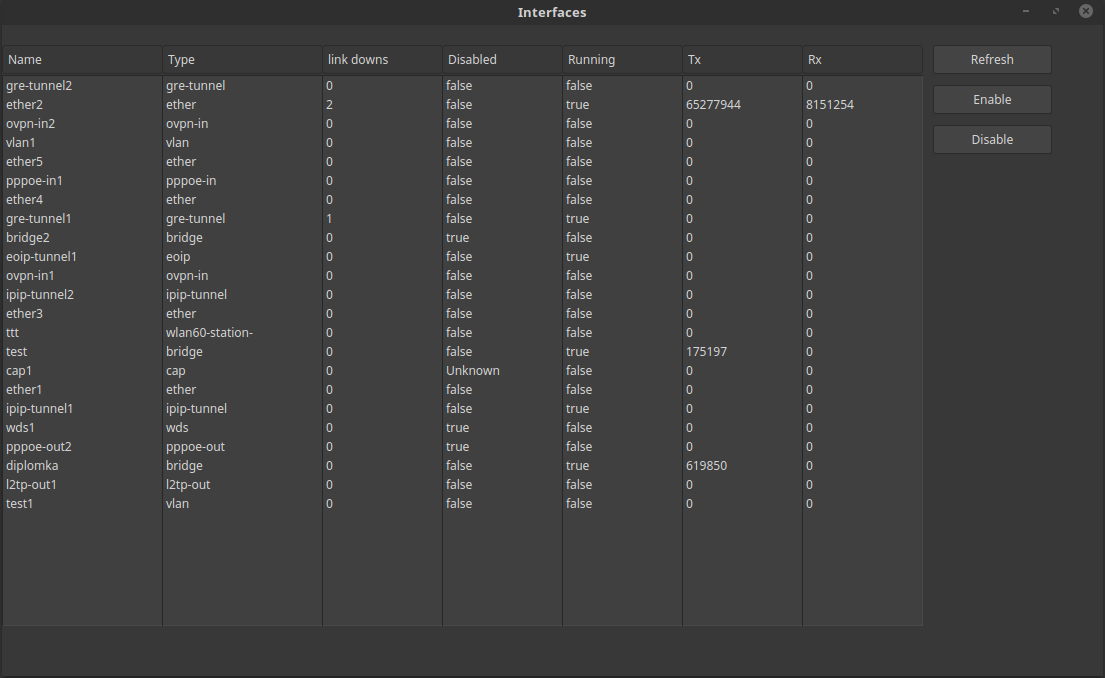
\includegraphics[scale=0.35]{../text/interfacesgui.png}
\caption{Okno interfaces}
\label{fig:interfacesgui}
\end{figure}
\begin{figure}[H]
\centering
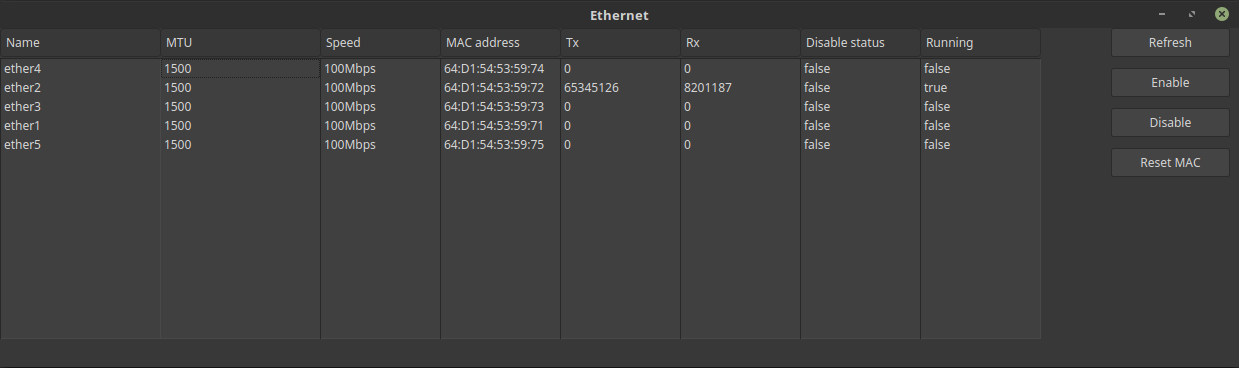
\includegraphics[scale=0.35]{../text/ethernet.png}
\caption{Okno ethernet}
\label{fig:ethernet}
\end{figure}
\begin{figure}[H]
\centering
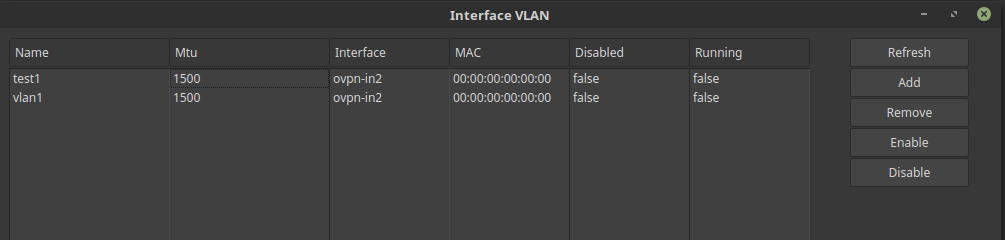
\includegraphics[scale=0.35]{../text/vlangui.png}
\caption{Okno VLAN}
\label{fig:vlangui}
\end{figure}
\begin{figure}[H]
\centering
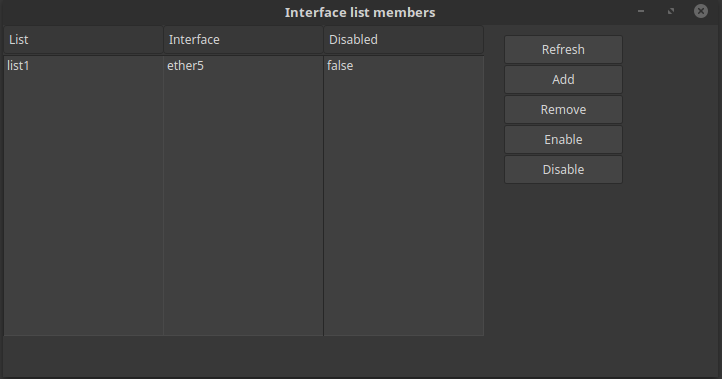
\includegraphics[scale=0.35]{../text/ifacelistmember.png}
\caption{Okno Interface list member}
\label{fig:interfacelistmembergui}
\end{figure}
\begin{figure}[H]
\centering
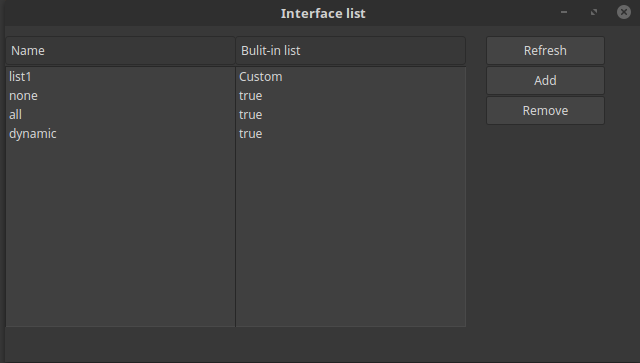
\includegraphics[scale=0.45]{../text/ifacelist.png}
\caption{Okno interface list}
\label{fig:interfacelistgui}
\end{figure}
\chapter{Návod na inštaláciu a spustenie}
\chapter{Testovanie aplikácie}


